\chapter{制冷}
\section{引言}
制冷对超导非常重要。对制冷的依赖性是超导广泛应用(如电力应用)的主要因素。然而,我们不以因为其重要性而过分强调它的作用。
单从制冷角度看,显然将超导磁体运行于最高的许可温度下是更高效的。但是,如果超导磁体是某系统的一部分,就必须评估运行温度对整个系统的影响。
“超导磁体的最佳运行温度”这个问题就成了现实且极端重要的设计/运行问题,对高温超导磁体尤其如此。比如,对运行于77K的超导磁体,如果产生
相同的磁场,无疑需要比运行于20K更多的超导体;制冷上的节省可能并不能补偿超导体费用的增加。

另一个不可忽略的是每一个超导系统的绝热要求:最好的绝热是真空。温度低于20K(氢的冰点)时,热学“有效”的真空在低温容器内是相对容易实现的。
已抽真空的低温容器表面逸出的氢气是容器内最主要的传热介质。于是,整个高温超导磁体系统若运行于20K之下(而不是之上)可能经济性更好。
如果我们选择一个更高的运行温度——比如很多人希望的~70K——系统中可能不再需要真空绝热,这时“干扰”又少了一点。

本部分,将简要讨论以下超导磁体的制冷设计、运行问题:1)两种超导体的冷却方式,“干式”和“湿式”;2)冷源、热源和制冷测量;
3)湿式磁体的制冷剂;4)可能对干式磁体有用的固体制冷剂。上述论题的更多细节将在“专题”部分有更深入的涉及和研究。

\section{“湿式”磁体和“干式”磁体}
在1990s前,所有的超导磁体都是“湿式”的,即靠液氦冷却。1990s早期开的,随着高温超导的发现以及制冷机技术的进步,由制冷机冷却的干式(无制冷剂)
LTS和HTS磁体都得以发展。一方面,干式低温系统在运行、维护上更轻便;另一方面,干式低温系统更易实现“少干扰”。这使得干式磁体在多数应用中是更优的
选项——如果磁体自身在正常运行条件下完全无耗散(如交流损耗)的话。

\subsection*{超导磁体的冷却方式}
如表4.1可见,超导磁体可以使用五种冷却方式(四种湿式和一种湿式)的任一种。尽管本节使用的“制冷??”、“绝热”、“准稳定性”等术语
在第六章会有更详细的讨论,但为了读者的可理解性,此处给出这些术语的简要定性解释。
\begin{description}
  \item[浸泡冷却cryostable?] 1980s以前建造的磁体基本都是浸泡式冷却的。这些磁体的一个关键制冷特征是为了便于制冷剂渗入的绕组的“通孔”设计。
  通孔让绕组的几乎所有部分都暴露于制冷工质。此时,下文定性讨论的对流传热是重要的。第六章会给出一些数据。
  \item[浸泡冷却绝热] 为了实现高性能,浸泡冷却的“绝热”磁体在1980s早期开始发展。此处,绕组是实心的,完全没有制冷剂的浸入。
  这样,绕组中的总体电流密度显著高于浸泡制冷??。绕组仅在其外表面被冷却。
  \item[迫冷cryostable] 为了保持制冷剂为单相(一般对浸泡式制冷磁体并不容易),以及为了加强绕组导体本身的强度,在1970s早期发展了所谓的“cable-in-conduit,CIC,特别是大型磁体”。此处,冷却和绕组高度耦合。重要的传热数据是哪些强迫对流参数。典型的传热数据在第六章给出。
  \item[迫冷准稳定性] 为了保持绕组鲁棒性,绕组上没有通孔。为实现比浸泡冷却绝热磁体更好的稳定性,制冷剂被强迫进入绕组。不是经由导体,而是
  仅在导体的临近边缘。和绝热绕组一样,导体是传导冷却的。
  \item[制冷机冷却] 磁体和制冷机相连;绕组内的冷却主要通过传导。如第六章将会更详细讨论的,LTS磁体运行于准稳定态,而HTS磁体运行于稳定态。
  “制冷循环器(cryocirculator)”对作为干式磁体冷源的制冷机是非常需要的,特别是对LTS磁体。
\end{description}
%%%表4.1
\begin{table}[htbp]\small
  \centering
  \caption{湿式和干式超导磁体的冷却方式} \label{coolingmethod}
\begin{tabular}{|c|c|c|}
  \hline
  % after \\: \hline or \cline{col1-col2} \cline{col3-col4} ...
\textbf{冷却方式}&\textbf{冷却-导体耦合性}&\textbf{传热方式} \\ \hline \hline
浸泡冷却,cryostable & 好;全部导体& 对流\\ \hline
浸泡冷却,绝热 & 基本不存在 &(磁体绕组表面的)传导 \\ \hline
迫冷,cryostable &好;全部导体&对流\\ \hline
迫冷,准稳定 &临近表面处,间接&传导\\ \hline\hline
制冷机,准稳定&间接 &传导 \\ \hline
\end{tabular}
\end{table}

\section{制冷问题:冷却、热、测量}
三个基本制冷问题是与超导磁体技术相关的:1)冷源;2)热源;3)测量。这些问题将在本部分简要讨论。专题部分以及后续章节将对某些特定问题
做更详细的讨论。
\subsection{冷源}
如表4.1总结的,超导磁体靠制冷工质或制冷机冷却并维持在其运行温度。下面将简明的讨论制冷剂。制冷机仅给出基本的热力学关系和性能数据。
\subsection{热源}
一般的,在超导磁体的低温容器内的冷环境中,主要有五个热源:1)低温容器壁间的辐射;2)低温容器壁间“真空”空间的热对流;3)磁体支撑和
低温容器结构单元的热传导;4)电流引线的传导和焦耳热耗散;5)磁体内的耗散。专题部分将会涉及到辐射、对流和电流引线。磁体的耗散将在第七章讨论。
\subsection{测量}
超导磁体运行中,通常测量的低温参数包括:1)温度;2)压力(低温容器真空度、工质压力);3)工质流速(迫冷湿式磁体);4)蒸发率(湿式磁体的电流引线)。本书中,专题部分仅涉及温度的测量简要讨论。

\section{液体工质:湿式磁体}
1990s前,仅液氦适用于磁体运行。某些液氦低温容器使用液氮来隔断热量。由于磁体要从室温冷却到4.2K,液氮也用于预冷液氦冷却磁体,以减少液氦的消耗。

大气压下饱和(沸腾)温度低于100K的6种工质是:氧(90.18K)、氩(87.28K)、氮(77.36K)、氖(27.09K)、氢(20.39K)、氦(4.22K)。
对于湿式高温超导磁体和设备,工质的备选顺序为氮、氖、氢。对于湿式低温超导或低温/高温混合磁体,如高场NMR磁体,仍然主要使用氦。五种
液体的沸腾热传递参数在表4.2列出。作为对比,还列出了水的参数。

%%表4.2
\begin{table}[htbp]\small
  \centering
  \caption{沸腾传热参数} \label{boilingpara}
\begin{tabular}{|c||c|c|c|c|c|}
  \hline
  % after \\: \hline or \cline{col1-col2} \cline{col3-col4} ...
\textbf{液体}&$T_a[K]$&$h_l[J/cm^3]$&$q_{pk}[W/cm^2]$&$\Delta T_{pk}[K]$&$q_{fm}[W/cm^2]$ \\ \hline \hline
氦&4.22&2.6&$\sim 1$&$\sim 1$&$\sim 0.3$\\ \hline
氢&20.39&31.3&$\sim 10$&$\sim 5$&$\sim 0.5$ \\ \hline
氖&27.09&104&$\sim 15$&$\sim 10$&$\sim 1$\\ \hline
氮&77.36&161&$\sim 25$&$\sim 15$&$\sim 2$\\ \hline
水&373.15&2255&$\sim 100$&$\sim 30$&$\sim 10$ \\ \hline
\end{tabular}
\end{table}

\subsection*{沸腾传热参数}
在湿式超导磁体中,特别是浸泡冷却cryostable磁体,冷却依靠核态沸腾传热。由于核态沸腾传热中,冷却是靠液体蒸发实现的,故液体的体积蒸发热$h_l$
是一个关键参数。这也意味着沸腾热流密度和温度的关系图像(两坐标轴均为对数坐标,如图\ref{boilingflux})对大多数液体都是看上去类似的。这里的x轴温度是浸入
液体的物体的避免温度和液体饱和温度之差,即$\Delta T=T-T_s$。图中的其他参数为:$q_{pk}$,最大核态沸腾热流密度;$\Delta T_{pk}$,是$q_{pk}$出现时的$\Delta T$;$q_{fm}$,最小膜态沸腾热流密度。

从表\ref{boilingpara}中我们可以得到,唯一适合LTS磁体的制冷剂液氦,蒸发时吸收的能量密度最小,是效果最差的。尽管HTS磁体最好是干式运行,但如果它湿式运行,
氢、氖、氮能够覆盖大多数HTS磁体的温度范围。燃料电池在电动汽车领域应用中发展出的一个重要成果就是液氢技术,包括安全性方面的技术。这可能会为
液氢冷却HTS磁体提供与有益促进。

%%%图4.1
\begin{figure}
  \centering
 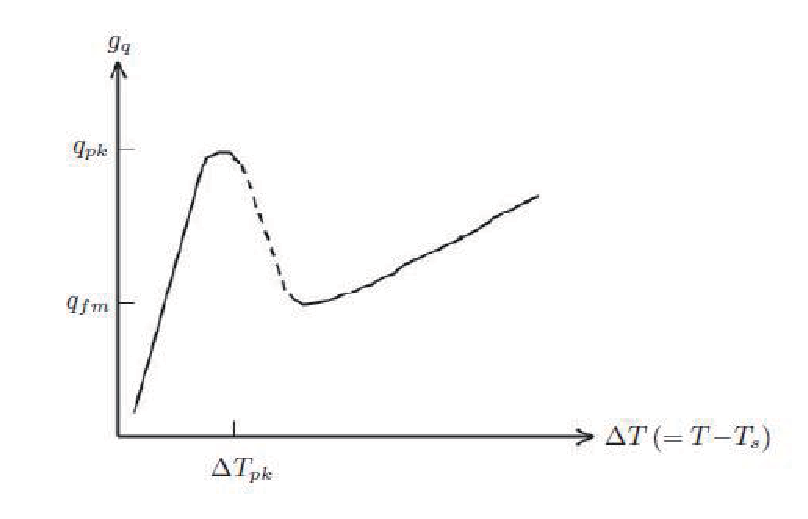
\includegraphics[scale=0.8]{chpt4/figs/fig4.1.eps}
  \caption{典型流体的沸腾热流密度 vs. 温度}\label{boilingflux}
\end{figure}

\section{固体工质:干式磁体}
正如前文所讲,干式低温磁体,特别是运行电流小于1kA的,很可能会逐渐替代湿式小电流LTS磁体。如果当前的高温超导体(BSCCO、YBCO和$MgB_2$)中
的一种、两种甚至三种发展为完全的“磁体级导体”,那在不久的将来,干式HTS磁体不仅会取代干式LTS磁体,还将找到仅适用于HTS磁体的其他应用。
\subsection{湿LTS磁体 vs. 干HTS磁体——热容}
湿式LTS磁体经常被忽略的一个优势是其巨大的热容,这是由作为湿式LTS磁体的一部分的大量液氦提供的。液氦的焓密度在4.2K时“高”达$2.6 J/cm^3$——
此处所谓高,是和铜相比的。铜在4.2-4.5K的焓密度仅为$\sim 0.0003J/cm^3$——是铜的1000倍。于是,在大多数情况下,液氦将牢牢将磁体的温度“铆”住。

干式磁体同样需要提供一个大的热容以便“铆”住温度。固态制冷剂是这种功能的很好选项。图\ref{fig:heatcap}给出了多种固体制冷剂(固氖、固氮、固氩)以及
部分金属(铅、银、铜)的热容和温度的关系。铅在低温设备中常用为热容增强部件;铜是LTS中广为使用的基底金属;银是BSCCO的基底金属。
%%%图4.2
\begin{figure}
  \centering
 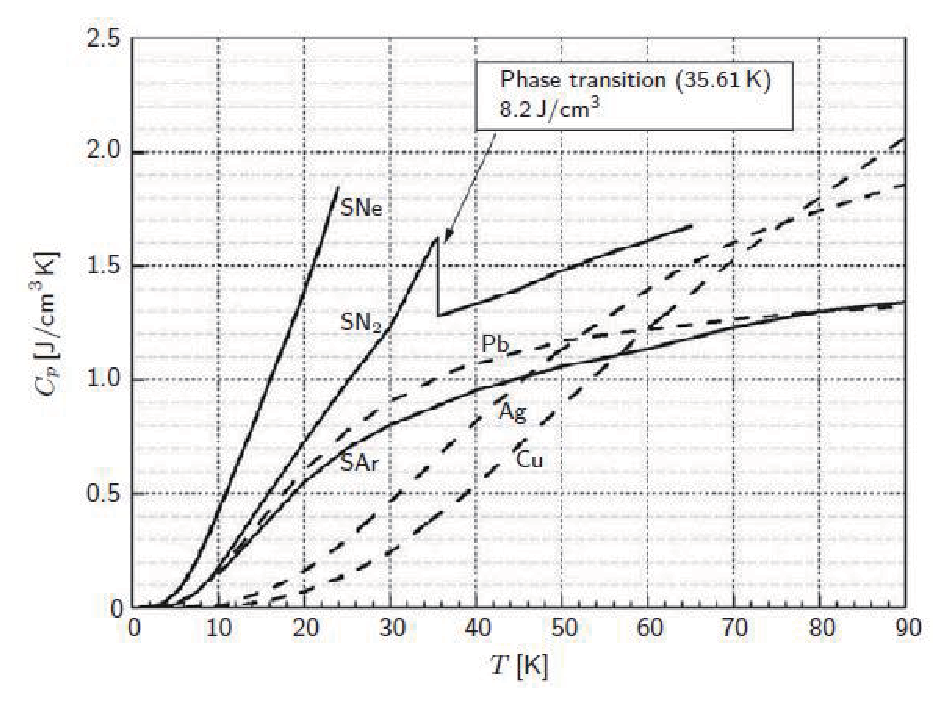
\includegraphics[scale=0.7]{chpt4/figs/fig4.2.eps}
  \caption{几种物质的热容$C_p$ vs. 温度T特性}\label{fig:heatcap}
\end{figure}

\subsection{固体工质——氖、氮、氩}
下面将简要讨论三种可能用于干式HTS磁体的固体工质:氖、氮、氩。附录中给出了他们的一些热力学性质。

尽管是高热容使得固体工质成为优秀的浸渍材料。此外,还有两个其他的性质让固体工质在一些应用中优于环氧:1)热导率;2)机械强度。在10-15K温度区间,
在HTS绕组上的温度均匀性上,固氮比环氧的效果更好。同时,固氮也使得绕组比环氧浸渍更具鲁棒性。

\begin{description}
  \item[固氮,$SN_2$] 因为它能在高达64.2K仍保持固态且不贵、重量很轻(铅的密度的1/10)、具有电绝缘性,固氮是运行于64K温度下温区的干式HTS磁体的
  有效热容增强剂。例如,BSCCO和YBCO磁体在20-60K温区肯定能运行;$MgB_2$磁体则是在10-15K甚至20-30K。从图4.2中看出,固氮在35.61K存在一个
  固-固态的相变,额外吸收能量$8.2J/cm^3$。由于在转变点古今的热容是约$1.5J/cm^3 K$,额外的$8.2J/cm^3$能量吸收等价于5K多的温升。对于运行于
  这个温区的HTS磁体,这是一个极佳的“温度池”。
  \item[固氖] 图4.2中的热容数据表明,固氖体积费用比固氮贵200倍,它将是4-10K温区的最佳热容增强剂。不过,10K左右时,固氮对于大多数情况就足够用了。
  尽管也有其他物质,比如$Er_3 Ni$,在4-24K温区能提供更好的热容增强效果。但是对磁体,固氖可能更合适。除了价格之外的最大缺点(相比于固氮),是
  固氖相对低的熔点,仅24.6K。这限制了固氖系统运行的温区。
  \item[固氩] 作为大气中含量最高的惰性气体,氩在价格上比氖至少便宜 一个数量级,不过比氮还是贵不少。固氩仅适用于运行于64.2K(固氮熔点)
  -83.8K(固氩熔点)温区的干式磁体。
\end{description}

\section{专题}
\subsection{题1:制冷机性能}

\newpage
\subsection{题2:湿式磁体的冷却模式}

\newpage
\subsection{题3:制冷高温超导磁体}

\newpage
\subsection{题4:超流}

\newpage
\subsection{题5:1.8K过冷}

\newpage
\subsection{题6:焦耳-汤姆森过程}

\newpage
\subsection{题7:制冷机 vs. 制冷循环机}

\newpage
\subsection{题8:辐射传热}

\newpage
\subsection{题9:残余气体的对流传热}

\newpage
\subsection{题10:真空泵系统}

\newpage
\subsection{题11:冷却固体工质/磁体}

\newpage
\subsection{题12:温升 vs. 场均匀性}

\newpage
\subsection{题13:低温量热计}

\newpage
\subsection{题14:蒸汽冷却的铜电流引线}

\newpage
\subsection{题15:干式引线:正常金属和HTS}

\newpage
\subsection{题16:电流引线保护}

\newpage
\subsection{题17:HTS电流引线}

\newpage
\subsection{题18:优化的CSV引线}

\newpage
\subsection{题19:气冷支撑棒}

\newpage
\subsection{题20:低温结构材料}